\documentclass{article}

\usepackage{libertine}

\usepackage{fontspec}
\setmainfont[Ligatures=TeX]{Ubuntu}

\usepackage[
    left=1in,
    right=1in,
    top=1in,
    bottom=1in
]{geometry}

\usepackage{fancyhdr}
\pagestyle{fancy}
\lhead{\href{https://github.com/QubitPi/old-persian}{Study Notes - Old Persian}}
\chead{\href{https://en.wikipedia.org/wiki/Old_Persian_cuneiform}{\scalebox{2}{\oldpersian pals}}}
\rhead{\href{https://github.com/QubitPi}{QubitPi}}
\lfoot{}
\cfoot{}
\rfoot{\thepage}

\renewcommand{\headrulewidth}{0.4pt}
\renewcommand{\footrulewidth}{0.4pt}

\usepackage{multicol}
\usepackage{graphicx}
\usepackage{float}
\graphicspath{ {./sections/img/} }
\usepackage{stackengine}
\usepackage{hyperref}
\hypersetup{
    colorlinks=true,
    linkcolor=blue,
    anchorcolor=blue,
    urlcolor=blue,
    citecolor=blue,
}

\newfontfamily{\oldpersian}{Parsoomash}

\setlength{\parindent}{0pt}


\begin{document}

    Old Persian is the name applied to the Persian language used in the cuneiform inscriptions of the Achaemenian dynasty; it can be localized as the langauge of southwestern Persia, or Persis in the narrower sense, and was the vernacular speech of the Achaemenian rulers.

    The Old Persian inscriptions are commonly accompanied also by translations into Elamite and Akkadian. Linguistically, Old Persian belongs to the Iranian branch of Indo-Iranian or Aryan, which is one of the main divisions of the Indo-European family of languages.

    \section{Writing System}\cite{OmniglotOldPersian,SkjærvøPersian}

Old Persian is written in a cuneiform script, but with only a small number of signs compared to languages such as
Akkadian. There are \hyperref[Vowel Signs]{3 vowel signs} and \hyperref[Consonant Signs]{33 consonant signs}

\subsection{Vowel Signs (3)}
\label{Vowel Signs}

\stackanchor{\scalebox{3}{\oldpersian a}}{\stackanchor{a}{\LKey{a}}} \space\space\space\space\space
\stackanchor{\scalebox{3}{\oldpersian i}}{\stackanchor{i}{\LKey{i}}} \space\space\space\space\space
\stackanchor{\scalebox{3}{\oldpersian u}}{\stackanchor{u}{\LKey{u}}} \space\space\space\space\space

\subsection{Consonant Signs (33)}
\label{Consonant Signs}

The consonant signs are syllabic, i.e.

\stackanchor{\scalebox{3}{\oldpersian k}}{\stackanchor{k/ka}{\LKey{k}}} \space\space\space\space\space
\stackanchor{\scalebox{3}{\oldpersian K}}{\stackanchor{ku}{\LKey{K}}} \space\space\space\space\space
\stackanchor{\scalebox{3}{\oldpersian x}}{\stackanchor{x/xa}{\LKey{x}}} \space\space\space\space\space
\stackanchor{\scalebox{3}{\oldpersian g}}{\stackanchor{g/ga}{\LKey{g}}} \space\space\space\space\space
\stackanchor{\scalebox{3}{\oldpersian G}}{\stackanchor{gu}{\LKey{G}}} \space\space\space\space\space
\stackanchor{\scalebox{3}{\oldpersian C}}{\stackanchor{c/ca}{\LKey{C}}} \space\space\space\space\space
\stackanchor{\scalebox{3}{\oldpersian c}}{\stackanchor{ç/ça}{\LKey{c}}} \space\space\space\space\space
\stackanchor{\scalebox{3}{\oldpersian j}}{\stackanchor{j/ja}{\LKey{j}}} \space\space\space\space\space
\stackanchor{\scalebox{3}{\oldpersian J}}{\stackanchor{ji}{\LKey{J}}} \space\space\space\space\space
\stackanchor{\scalebox{3}{\oldpersian t}}{\stackanchor{t/ta}{\LKey{t}}} \space\space\space\space\space
\stackanchor{\scalebox{3}{\oldpersian T}}{\stackanchor{tu}{\LKey{T}}} \space\space\space\space\space
\stackanchor{\scalebox{3}{\oldpersian o}}{\stackanchor{θ/θa}{\LKey{o}}} \space\space\space\space\space
\stackanchor{\scalebox{3}{\oldpersian d}}{\stackanchor{d/da}{\LKey{d}}} \space\space\space\space\space
\stackanchor{\scalebox{3}{\oldpersian D}}{\stackanchor{di}{\LKey{D}}} \space\space\space\space\space
\stackanchor{\scalebox{3}{\oldpersian ?}}{\stackanchor{du}{\LKey{question}}} \space\space\space\space\space
\stackanchor{\scalebox{3}{\oldpersian P}}{\stackanchor{p/pa}{\LKey{P}}} \space\space\space\space\space
\stackanchor{\scalebox{3}{\oldpersian f}}{\stackanchor{f/fa}{\LKey{f}}} \space\space\space\space\space
\stackanchor{\scalebox{3}{\oldpersian b}}{\stackanchor{b/ba}{\LKey{b}}} \space\space\space\space\space
\stackanchor{\scalebox{3}{\oldpersian n}}{\stackanchor{n/na}{\LKey{n}}} \space\space\space\space\space
\stackanchor{\scalebox{3}{\oldpersian N}}{\stackanchor{n/nu}{\LKey{N}}} \space\space\space\space\space
\stackanchor{\scalebox{3}{\oldpersian m}}{\stackanchor{m/ma}{\LKey{m}}} \space\space\space\space\space
\stackanchor{\scalebox{3}{\oldpersian M}}{\stackanchor{mi}{\LKey{M}}} \space\space\space\space\space
\stackanchor{\scalebox{3}{\oldpersian ,}}{\stackanchor{mu}{\LKey{comma}}} \space\space\space\space\space
\stackanchor{\scalebox{3}{\oldpersian y}}{\stackanchor{y/ya}{\LKey{y}}} \space\space\space\space\space
\stackanchor{\scalebox{3}{\oldpersian v}}{\stackanchor{v/va}{\LKey{v}}} \space\space\space\space\space
\stackanchor{\scalebox{3}{\oldpersian V}}{\stackanchor{vi}{\LKey{V}}} \space\space\space\space\space
\stackanchor{\scalebox{3}{\oldpersian r}}{\stackanchor{r/ra}{\LKey{r}}} \space\space\space\space\space
\stackanchor{\scalebox{3}{\oldpersian R}}{\stackanchor{ru}{\LKey{R}}} \space\space\space\space\space
\stackanchor{\scalebox{3}{\oldpersian l}}{\stackanchor{l/la}{\LKey{l}}} \space\space\space\space\space
\stackanchor{\scalebox{3}{\oldpersian s}}{\stackanchor{s/sa}{\LKey{s}}} \space\space\space\space\space
\stackanchor{\scalebox{3}{\oldpersian S}}{\stackanchor{š/ša}{\LKey{S}}} \space\space\space\space\space
\stackanchor{\scalebox{3}{\oldpersian z}}{\stackanchor{z/za}{\LKey{z}}} \space\space\space\space\space
\stackanchor{\scalebox{3}{\oldpersian h}}{\stackanchor{h/ha}{\LKey{h}}} \space\space\space\space\space

\subsection{Logograms (Signs That Stand for a Whole Word)}

\stackanchor{\scalebox{3}{\oldpersian Q}}{\stackanchor{king}{\LKey{Q}}} \space\space\space\space\space
\stackanchor{\scalebox{3}{\oldpersian e}}{\stackanchor{earth}{\LKey{e}}} \space\space\space\space\space
\stackanchor{\scalebox{3}{\oldpersian 43}}{\stackanchor{country}{\LKey{4}\LKey{3}}} \space\space\space\space\space
\stackanchor{\scalebox{3}{\oldpersian 6}}{\stackanchor{god}{\LKey{6}}} \space\space\space\space\space
\stackanchor{\scalebox{3}{\oldpersian Wq}}{\stackanchor{Ahuramazada}{\LKey{W}\LKey{q}}} \space\space\space\space\space
\stackanchor{\scalebox{3}{\oldpersian q}}{\stackanchor{Ahuramazada (genitive)}{\LKey{q}}} \space\space\space\space\space

    \section{Behistun Inscription}

\begin{figure}[H]
    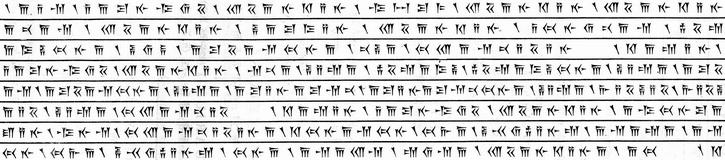
\includegraphics[width=\textwidth]{column-i-lines-1-8}
    \caption{Behistun Inscription, Column i, lines 1-8\cite{BehistunT01}}
\end{figure}

\begin{enumerate}
    \item {\oldpersian ;}\stackunder{{\oldpersian adm}}{(Pronoun) I\cite{adm}} {\oldpersian ;} \stackunder{{\oldpersian daryvuS}}{Darius\textsuperscript{\cite[p185]{rawlinson1849memoir}}\cite{darius}}{\oldpersian ;} \stackunder{\oldpersian xSsayoiy}{Alternative form of {\oldpersian Q}\cite{alternativeKing}} {\oldpersian ;} \stackunder{{\oldpersian vzrk}}{great\cite{great}} {\oldpersian ;} {\oldpersian xSsayoiy} {\oldpersian ;} {\oldpersian xSsayoiyanam} {\oldpersian ;} {\oldpersian xSsayoiy} {\oldpersian ;} {\oldpersian parsiy} {\oldpersian ;} {\oldpersian xSsayoiy} {\oldpersian ;} {\oldpersian ihyunam}
\end{enumerate}

\begin{enumerate}
    \item I am Darius, the great king, king of kings, the king of Persia, the king of countries, the son of Hystaspes,
         the grandson of Arsames, the Achaemenid.
    \item King Darius says: My father is Hystaspes; the father of Hystaspes was Arsames; the father of Arsames was
          Ariaramnes; the father of Ariaramnes was Teispes; the father of Teispes was Achaemenes.
    \item King Darius says: That is why we are called Achaemenids; from antiquity we have been noble; from antiquity
          has our dynasty been royal.
\end{enumerate}

    \section{Typing Old Persian}\cite{TypePersian}

\begin{multicols}{4}
    \count255=32
    \loop\ifnum\count255<125
    \advance\count255 1
    \hbox{\hbox to 1em{\symbol{\count255}\hss}\hbox{\oldpersian\symbol{\count255}}}
    \repeat
\end{multicols}


    \bibliographystyle{plain}
    \nocite{*}
    \bibliography{refs}

\end{document}
